\subsubsection{Compito C3: Pianificare un esame}

Il compito C3 richiedeva all'utente di pianificare un nuovo esame denominato "Architettura" con data 22/09/2026, associando un'attività specifica ("Riassumere il primo capitolo") e collegando al piano di studio il documento "Appunti\_Lezione.pdf" caricato nel compito precedente. L'obiettivo era valutare l'usabilità del sistema di organizzazione dello studio, con particolare attenzione ai percorsi di navigazione verso la sezione dedicata agli esami e all'intuitività dell'interfaccia per la gestione dei task e dei materiali allegati.

\paragraph{Analisi delle prestazioni generali}

Come si può notare dai dati aggregati per il compito C3 (Tabella~\ref{tab:6-c3-1}), il tasso di completamento (Success Rate) si è attestato al 100,00\% per entrambe le versioni del sistema. La versione post-riprogettazione (B) evidenzia miglioramenti su tutte le metriche considerate: la media degli errori si riduce del 57,14\% (da 0,93 a 0,40) e la mediana dei click diminuisce del 34,78\% (da 23 a 15). Si osserva inoltre una riduzione del 21,05\% nel tempo mediano di esecuzione e un calo del 29,27\% nella difficoltà percepita dagli utenti.

\begin{figure}[H]
	\centering
	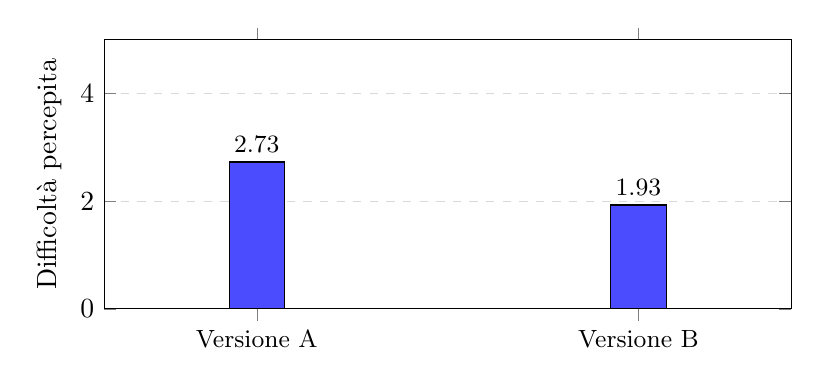
\begin{tikzpicture}
		\begin{axis}[
				ybar,
				bar width=20pt,
				width=0.85\textwidth,
				height=5cm,
				symbolic x coords={Versione A, Versione B},
				xtick=data,
				x tick label style={font=\small},
				ylabel={Difficoltà percepita},
				ymin=0, ymax=5,
				ymajorgrids=true,
				grid style={dashed, gray!30},
				enlarge x limits=0.4,
				nodes near coords,
				every node near coord/.style={font=\small, color=black},
			]
			\addplot+[
				ybar,
				fill=blue!70,
				draw=black
			] coordinates {
					(Versione A,2.73)
					(Versione B,1.93)
				};
		\end{axis}
	\end{tikzpicture}
	\caption{Confronto della difficoltà percepita tra Versione A e Versione B per C3.}
	\label{fig:6-c3-1}
\end{figure}

\begin{table}[H]
	\centering
	\footnotesize
	\renewcommand{\arraystretch}{1.2}
	\caption{Metriche prestazionali globali aggregate per il compito C3.}
	\label{tab:6-c3-1}
	\begin{tabular}{|>{\raggedright\arraybackslash}p{2.2cm}|>{\centering\arraybackslash}p{1.5cm}|>{\centering\arraybackslash}p{1.5cm}|>{\centering\arraybackslash}p{1.5cm}|>{\centering\arraybackslash}p{1.5cm}|>{\centering\arraybackslash}p{1.8cm}|>{\centering\arraybackslash}p{1.6cm}|}
		\hline
		\rowcolor{gray!30}
		\textbf{C3}           & \multicolumn{2}{c|}{\textbf{Versione A}} & \multicolumn{2}{c|}{\textbf{Versione B}} & \textbf{Variazione \%} & \textbf{Rilevanza}                                            \\ \hline
		\textit{Success Rate} & \multicolumn{2}{c|}{100,00\%}            & \multicolumn{2}{c|}{100,00\%}            & \textbf{Invariato}     &                                                               \\ \hline
		\rowcolor{gray!30}
		                      & \textbf{Media}                           & \textbf{DEV.ST}                          & \textbf{Media}         & \textbf{DEV.ST}    & \multicolumn{2}{c|}{}                    \\ \hline
		\textit{Errori}       & 0,93                                     & 1,22280                                  & 0,400                  & 0,73679            & \textbf{-57,14\%}     & \pvalue{0,13496} \\ \hline
		\textit{Tempo}        & 2.15.28                                  & 0,04102                                  & 1.43.08                & 0,02792            & \textbf{-23,87\%}     & \pvalue{0,05534} \\ \hline
		\textit{Click}        & 24,47                                    & 6,77038                                  & 14,20                  & 3,14416            & \textbf{-41,96\%}     & \pvalue{0,00014} \\ \hline
		\rowcolor{gray!30}
		                      & \multicolumn{2}{c|}{\textbf{Mediana}}    & \multicolumn{2}{c|}{\textbf{Mediana}}    & \multicolumn{2}{c|}{}                                                                  \\ \hline
		\textit{Difficoltà}   & \multicolumn{2}{c|}{3}                   & \multicolumn{2}{c|}{2}                   & \multicolumn{2}{c|}{}                                                                  \\ \hline
	\end{tabular}
\end{table}

La riduzione dei tempi, dei click e del tasso di errore indica che il redesign ha migliorato la navigabilità del sistema e la visibilità della sezione dedicata agli esami. La riorganizzazione dell’interfaccia e la semplificazione dei percorsi di accesso hanno consentito una maggiore immediatezza nell’esecuzione del compito e una riduzione del carico cognitivo.

\paragraph{Analisi qualitativa: commenti e osservazioni degli utenti}

I risultati quantitativi trovano riscontro nelle osservazioni qualitative e nei commenti raccolti. Per la versione originale (A), sono emerse criticità ricorrenti:

\begin{itemize}
	\item \textbf{Disorientamento e terminologia poco chiara}: la navigazione è risultata difficoltosa a causa dell’uso dell’etichetta "StudyFlow AI" per la sezione dedicata agli esami. Tale denominazione è stata frequentemente percepita come poco rappresentativa della funzionalità, generando incertezza nell’individuazione della sezione corretta.

	\item \textbf{Architettura dell’informazione poco coerente}: l’interfaccia è stata descritta come poco lineare, con molteplici modi per eseguire le stesse operazioni. In particolare, la necessità di passare dalla dashboard principale per creare un nuovo esame è stata percepita come un passaggio non necessario, portando in alcuni casi all’utilizzo della dashboard come punto di accesso alternativo.

	\item \textbf{Scarsa visibilità dei controlli}: anche la funzione di associazione dei materiali di studio ha presentato difficoltà di individuazione, risultando poco evidente e non immediatamente accessibile.
\end{itemize}

Per la versione post-riprogettazione (B), i risultati indicano un miglioramento generale dell’esperienza, pur con alcuni margini residui di ottimizzazione:

\begin{itemize}
	\item \textbf{Maggiore chiarezza della navigazione}: l’interfaccia è stata percepita come più semplice e coerente. L’accesso diretto alla sezione "Esami" ha ridotto le difficoltà di individuazione della funzionalità rispetto alla versione precedente.

	\item \textbf{Affinamenti necessari nei micro-flussi}: nonostante il miglioramento complessivo, alcuni utenti hanno segnalato incertezze nella gestione delle attività secondarie. In particolare, l’uso di un’icona a freccia per la rimozione di un task è stato talvolta ritenuto poco intuitivo.
\end{itemize}

\paragraph{Valutazione dell'effetto di apprendimento}

Analizzando i dati in base all'ordine di esecuzione (Tabella~\ref{tab:6-c3-2}) risulta chiaro che, in questo caso, l'esperienza pregressa dell'utente conta meno rispetto alla struttura dell'interfaccia.

Nel gruppo A--B, il tempo mediano di esecuzione passa da 1:53 (versione A) a 1:27 (versione B), con una riduzione del 23,01\%.

Nel gruppo B--A, gli utenti completano inizialmente il compito sulla versione B in 1:46,5, mentre nella successiva interazione con la versione A il tempo mediano aumenta fino a 2:02. Questo risultato suggerisce che l’esperienza maturata con la versione più ottimizzata non si trasferisce in modo efficace alla versione originale, le cui criticità strutturali continuano a incidere in maniera significativa sulle prestazioni, indipendentemente dalla familiarità con il task.

\begin{table}[H]
	\centering
	\footnotesize
	\renewcommand{\arraystretch}{1.2}
	\caption{Confronto delle metriche prestazionali in funzione dell'ordine di esecuzione per il compito C3.}
	\label{tab:6-c3-2}
	\begin{tabular}{|>{\raggedright\arraybackslash}p{2.2cm}|>{\centering\arraybackslash}p{1.0cm}|>{\centering\arraybackslash}p{1.0cm}|>{\centering\arraybackslash}p{1.8cm}|>{\centering\arraybackslash}p{1.6cm}|>{\centering\arraybackslash}p{1.0cm}|>{\centering\arraybackslash}p{1.0cm}|>{\centering\arraybackslash}p{1.8cm}|>{\centering\arraybackslash}p{1.6cm}|}
		\hline
		\rowcolor{gray!30}
		\textbf{Metrica}              & \multicolumn{4}{c|}{\textbf{Ordine A--B}}                                                 & \multicolumn{4}{c|}{\textbf{Ordine B--A}}                                                 \\ \cline{2-9} 
		\rowcolor{gray!30}
		                              & \textbf{A}          & \textbf{B}          & \textbf{Variazione \%} & \textbf{Rilevanza}        & \textbf{B}          & \textbf{A}          & \textbf{Variazione \%} & \textbf{Rilevanza}        \\ \hline
		\textit{Tempo (Media)}        & 2.14.20             & 1.31.20             & \textbf{-32,01\%}      & \pvalue{0,02105}          & 2.00.50             & 2.17.10             & \textbf{13,52\%}       & \pvalue{0,40930}          \\ \hline
		\textit{Errori (Media)}       & 1,22                & 0,667               & \textbf{-45,45\%}      & \pvalue{0,21446}          & 0,000               & 0,50                & \textbf{Invariato}     & \pvalue{0,20311}          \\ \hline
		\textit{Click (Media)}        & 22,22               & 14,89               & \textbf{-33,00\%}      & \pvalue{0,00442}          & 13,17               & 27,83               & \textbf{111,39\%}      & \pvalue{0,00755}          \\ \hline
		\textit{Difficoltà (Mediana)} & 2                   & 1                   &                        & \pvalue{}                 & 2                   & 3,5                 &                        & \pvalue{}                 \\ \hline
	\end{tabular}
\end{table}

Le stesse criticità si riflettono sulle valutazioni di difficoltà riassunte nella Figura~\ref{fig:6-c3-2}. Nel gruppo B–A si nota lo stacco più evidente: gli utenti che iniziano con la Versione B assegnano un punteggio di 2,00, ma al successivo passaggio alla versione originale (A) la difficoltà percepita aumenta sensibilmente, raggiungendo un valore di 3,50. Questo valore dimostra che, dopo aver utilizzato la versione chiara, l'impatto con l'etichetta "StudyFlow AI" e i passaggi forzati dalla dashboard della versione A diventa ancora più frustrante. Nel gruppo A--B, invece, la variazione è stata inferiore alle aspettative (da 2,22 a 1,89), simbolo che aver affrontato prima la versione complicata ha aiutato gli utenti a capire come funzionava la piattaforma, rendendo poi il passaggio alla versione B più morbido, anche se i piccoli difetti rimasti (come la freccia poco intuitiva per cancellare i task) hanno impedito al punteggio di scendere ancora di più.

\begin{figure}[H]
	\centering
	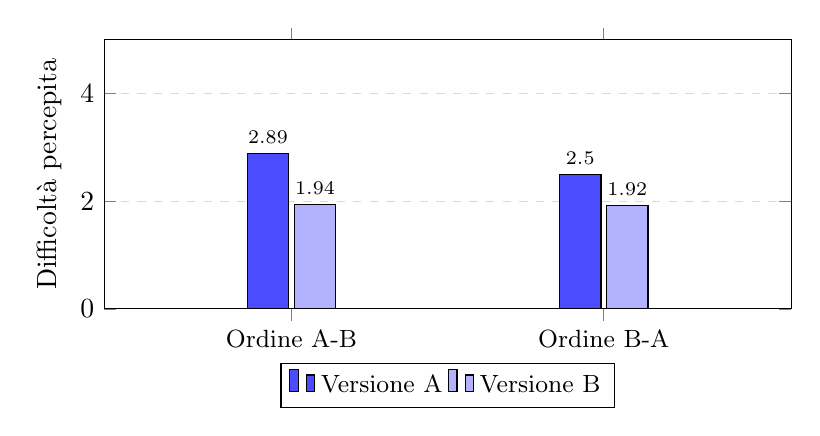
\begin{tikzpicture}
		\begin{axis}[
				ybar,
				bar width=15pt,
				width=0.85\textwidth,
				height=5cm,
				symbolic x coords={Ordine A-B, Ordine B-A},
				xtick=data,
				x tick label style={font=\small},
				ylabel={Difficoltà percepita},
				ymin=0, ymax=5,
				ymajorgrids=true,
				grid style={dashed, gray!30},
				enlarge x limits=0.6,
				legend style={at={(0.5,-0.2)}, anchor=north, legend columns=-1, font=\small},
				nodes near coords,
				every node near coord/.append style={font=\scriptsize, color=black},
			]
			\addplot+[
				fill=blue!70,
				draw=black
			] coordinates {
					(Ordine A-B,2.89)
					(Ordine B-A,2.50)
				};
			\addplot+[
				fill=blue!30,
				draw=black
			] coordinates {
					(Ordine A-B,1.94)
					(Ordine B-A,1.92)
				};
			\legend{Versione A, Versione B}
		\end{axis}
	\end{tikzpicture}
	\caption{Confronto della difficoltà percepita tra Versione A e Versione B per C3 in base all'ordine di esecuzione.}
	\label{fig:6-c3-2}
\end{figure}
